\section{Assembly component}

\textbf{Created by:} Dušan Šormaz \\
\textbf{Modified by:}  \\

address all times/ sometimes and also transitivity of these two pairs of relationships.

\subsection*{Scenario Objective}
From Arko's email, 1/7/25 
I want to mention that however we are showing the basic use of "component part of" relation for expressing parthood, we should also show the use of "at some time" vs. "at all times" under this scenario. Also, the nuanced semantics of "component of at all times" vs. "has component at all times" (explain why they are not inverses to each other) is to be examined.
DNS
We also need to show multiple levels of assemblies, at least three. Should we consider assembly process(es)? 


\subsection*{General Pattern Description}

\sloppy This scenario shows uses of \opname{iof}{componentPartOf}, \opname{bfo}{continuantPartofAtSomeTime}, and \opname{bfo}{continuantPartofAtAllTimes} object properties. The general pattern is shown in fig. 15. The figure shows that an artifact in the product role may be assembly when it consists of components that are assembled to form a functional unit. In general, an assembled product consists of several levels of components, some of which may be assemblies, and some just simple mechanical parts. Both of those categories play the role of a MaterialComponentRole. The relations between an assembly and its component may be of two kinds: a) permanent, such as for welded (or similar processes) assemblies, in which case we need to use the \opname{iof}{hasComponentAtAllTimes} relation, or b) temporal, with an option of later disassembly (for example, for repair or replacement), usually assembled with some  kind of fasteners (bolts, nuts, etc.), in which case we need to use the \opname{iof}{hasComponentAtSomeTime} relation.

example car is salvaged and engine is kept for us in the other car. 
another example is in welding it is permanent, you have to throw away both welded parts. 
use example of the car to illustrate reasoning and its difference in AllTimes and SomeTimes

\begin{figure}
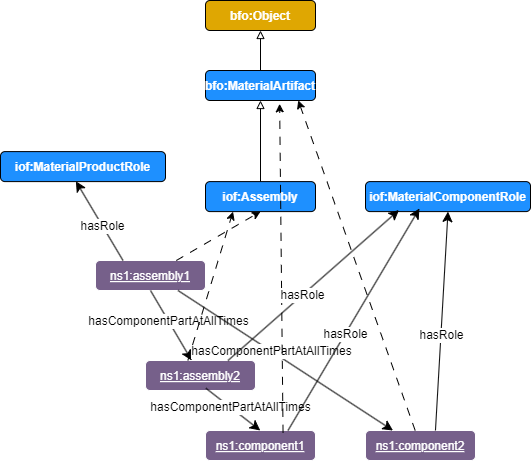
\includegraphics[scale=0.5]{scenarios/assemblies-components/images/assembly-components-generic.png}
\caption{The general pattern for the use of component-related object properties} 
\label{gen-pttn-components}
\end{figure}


\subsection*{Examples}

A car engine is often showcased in parts: pistons, crankshaft, and cylinders.

An insulated wall comprises drywall, insulation foam, and outer sheathing.

Sewing patches of silk, cotton and leather make an item of clothing.
\subsubsection*{Mechanical vise}
This example demonstrates how to model simple mechanical assemblies or devices. In this case we have a simple mechanical vise, designed in the CAD system (ref siemens), see figure ???. It consists of two jaw assemblies, fixed jaw and moving jaw. They are connected by the guide which allows the moving jaw to slides for desired distance.
\begin{figure}
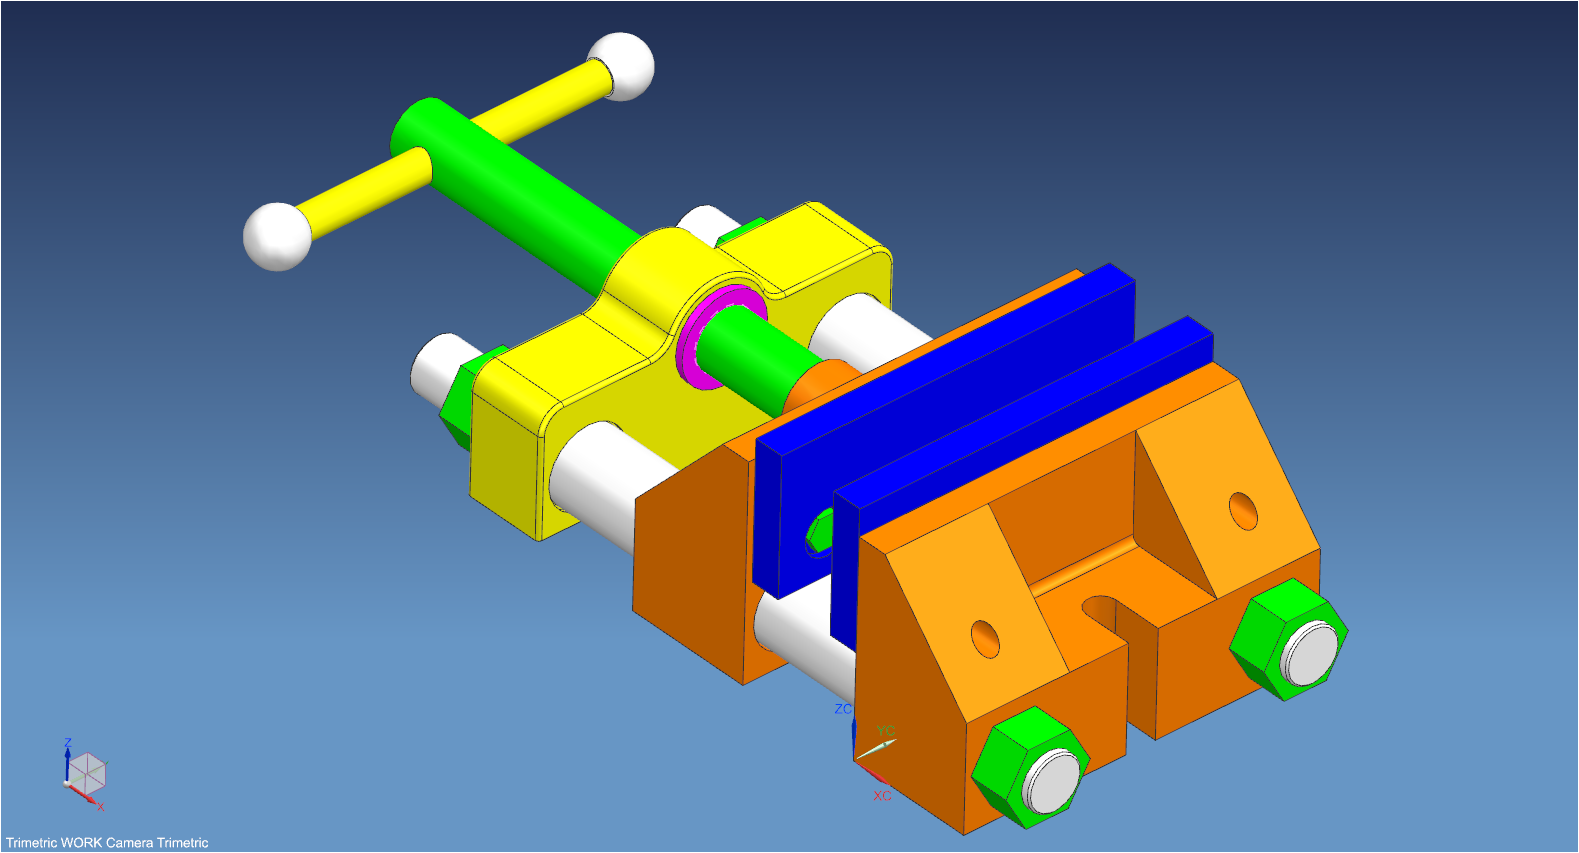
\includegraphics[scale=0.2]{scenarios/assemblies-components/images/dau_vise_assm.png}
\caption{Solid model of vise and its components} 
\label{vise-assmebly-model}
\end{figure}
\begin{figure}
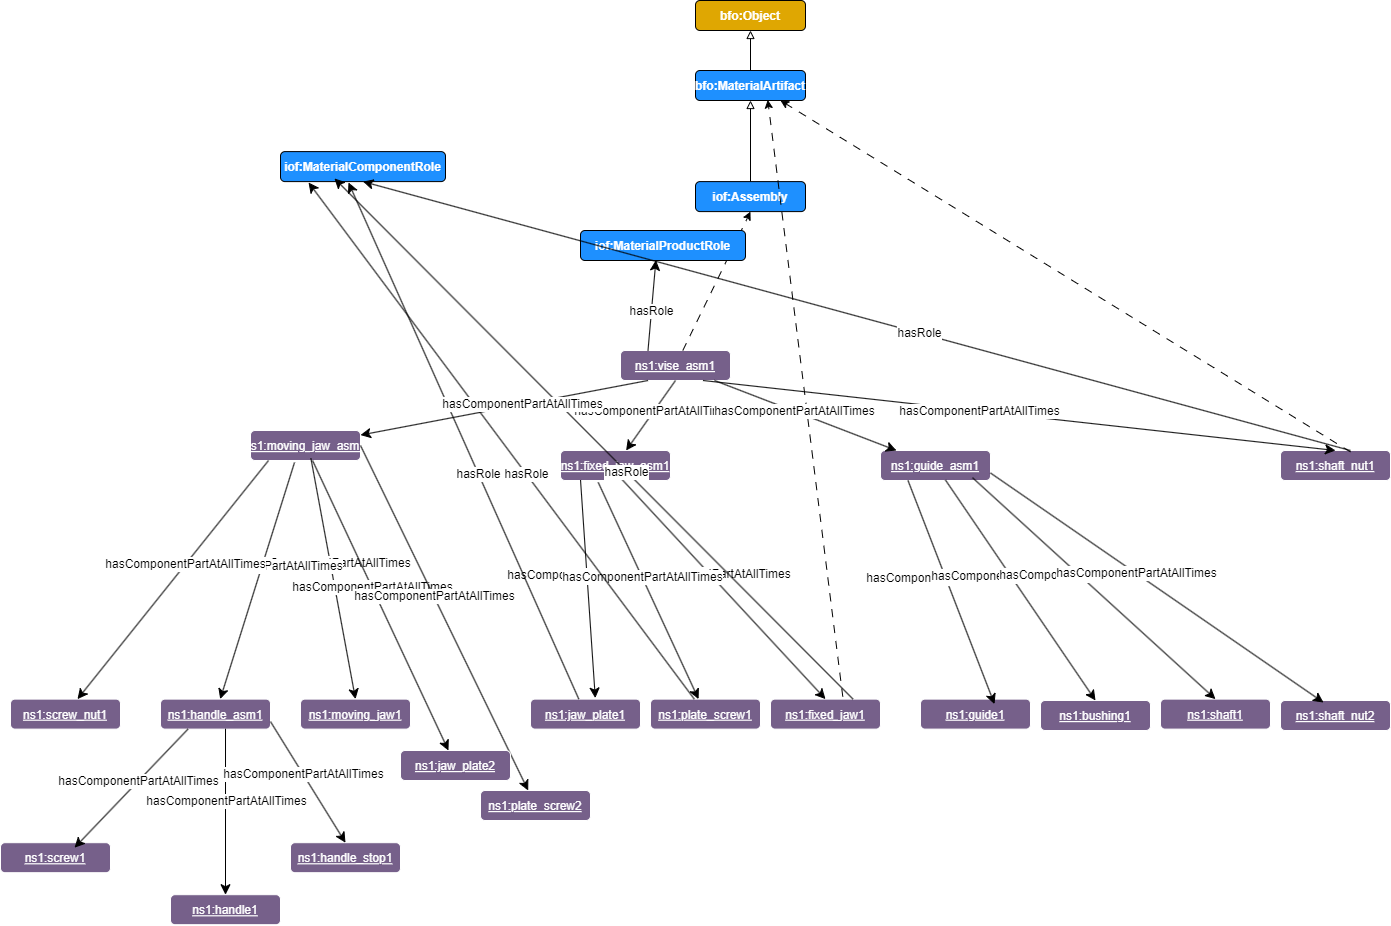
\includegraphics[scale=0.2]{scenarios/assemblies-components/images/vise-asembly-component.png}
\caption{The use of the general pattern in modeling the vise and its components} 
\label{vise-assmebly-components}
\end{figure}

% \section{Embedded components}

% Reinforcement Bars in Concrete Structures

% coating on a metal surface - this is not assembly

% printed circuit on board

% Embedded sensors